De opeenvolgende waarden van de benaderingsfout $\lVert f-z_{mn} \rVert_2$ voor $m = n = 1,\dots,20$ voor beide datasets van opgave 2 worden weergegeven in figuur~\ref{fig:oef13}. We zien hier duidelijk dat voor de tweede dataset veeltermoppervlakken een geschikte benadering is. De eerste dataset heeft een slechte veeltermbenadering voor kleine $m,n$. Dat komt omdat de fuctie $f(x,y)=sin((2x-1)^2+2y)$ een zekere periodiciteit bevat en kan dus beter benaderd worden door middel van trigonometrische functies.

\begin{figure}[H]
    \centering
    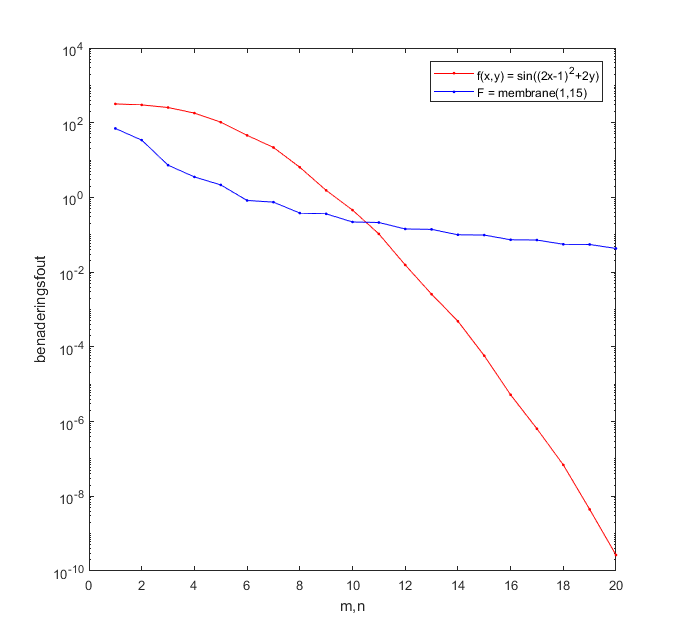
\includegraphics[width=0.5\textwidth]{oef13.png}
    \caption{benaderingsfout $\lVert f-z_{mn} \rVert_2^2$ van de veeltermbenadering van de functie $f(x,y)=sin((2x-1)^2+2y)$ en $F=\texttt{membrane}(1,15)$ in functie van de graad in $x$ en $y$}
    \label{fig:oef13}
\end{figure}